%!TEX encoding = IsoLatin

%% Document is article 
\documentclass[a4paper]{article}

%% ----------------------------------------------------- PACKAGES ----------------------------------------------------- %%
\usepackage{coolArticle}
\usepackage{caption}

%% ---------------------------------------------------- DOCUMENT ---------------------------------------------------- %%
\begin{document}

\noindent \textsc{Gallois-Montbrun} Gr�goire\\
\textsc{Faury} Louis 
	\titlebox{0.6}{Model Predictive Control}{Exercise \#2 - \textcolor{blue}{Group 2}}
	
	\section{Exercise 1}
	{
		\paragraph{} We implemented the Barrier method using the pseudo-code given in the exercise sheet. We provide here four illustrations of convergence toward a feasible optimum, for randomly generated QP problems, with inequality constraints. 
		
		\begin{figure}[h!]
			\begin{minipage}{0.5\linewidth}
				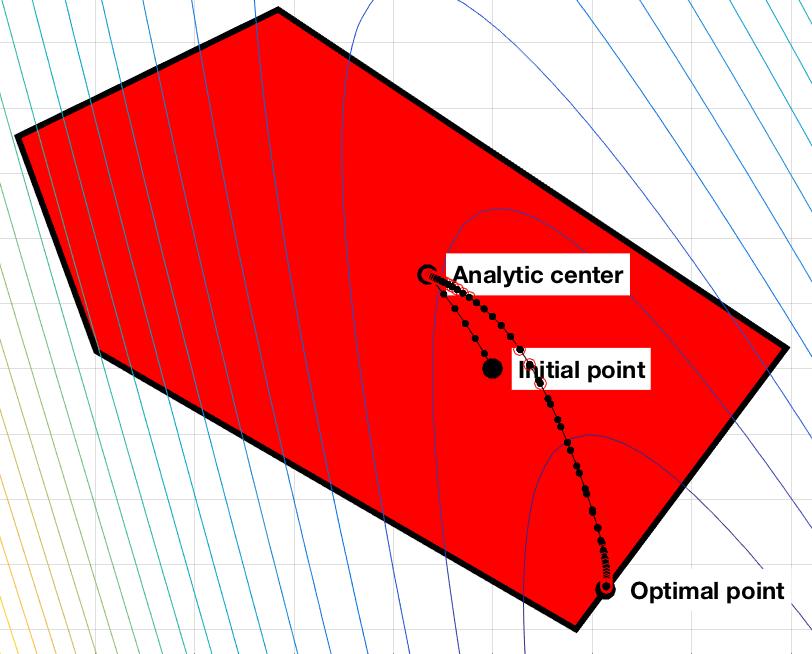
\includegraphics[width=0.9\linewidth]{1_mue-2}
				\caption{First example $\mu = 10^{-2}$}
			\end{minipage}
			\begin{minipage}{0.5\linewidth}
				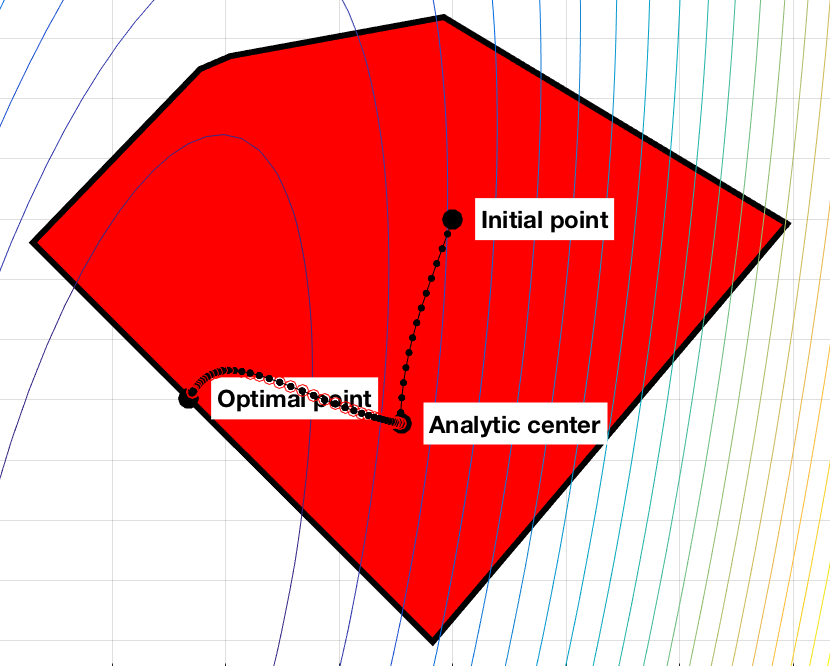
\includegraphics[width=0.9\linewidth]{2_mue-2}
				\caption{Second example $\mu = 10^{-2}$}	
			\end{minipage}
		\end{figure}
		
		\begin{figure}[h!]
			\begin{minipage}{0.5\linewidth}
				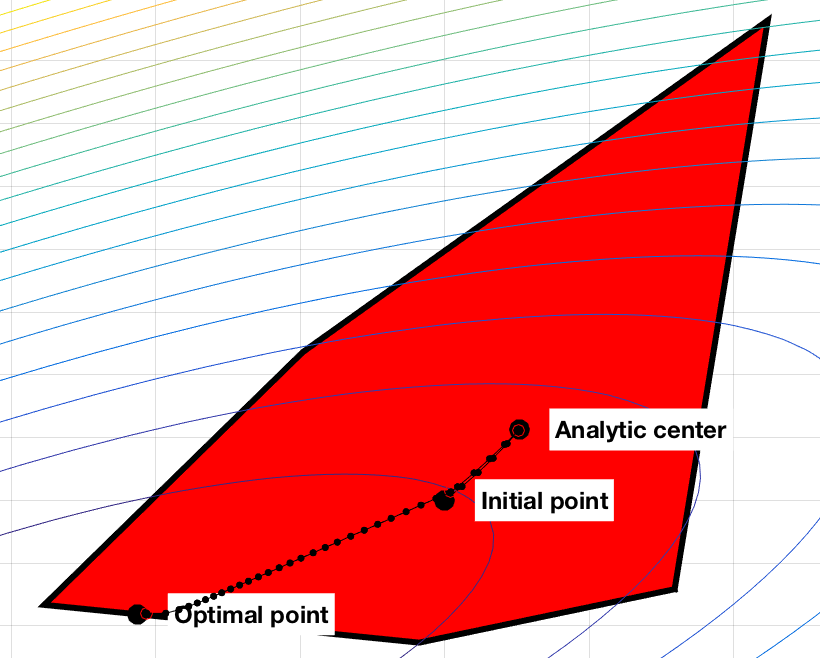
\includegraphics[width=0.9\linewidth]{1_mu5e-3}
				\caption{First example $\mu = 5*10^{-2}$}
				\label{n12}
			\end{minipage}
			\begin{minipage}{0.5\linewidth}
				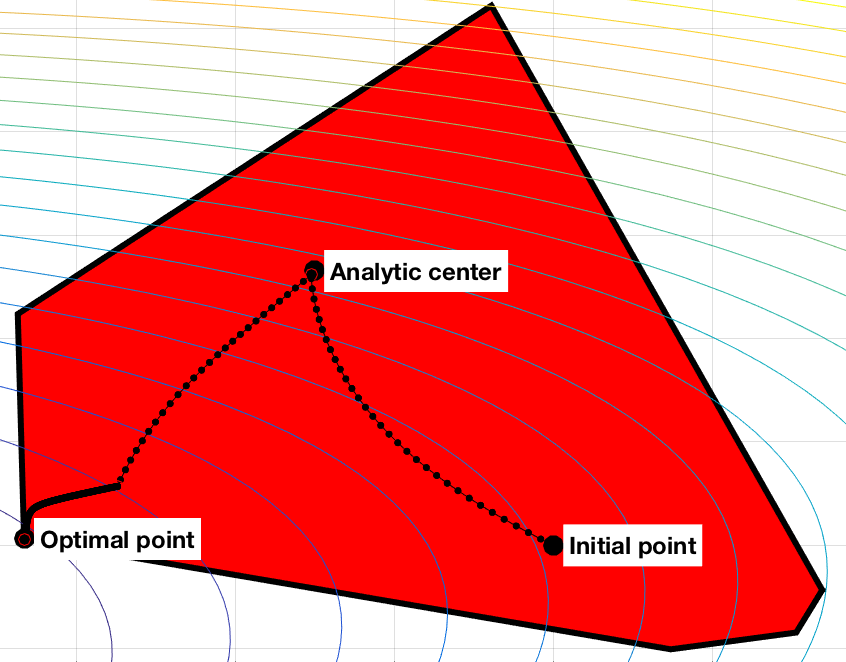
\includegraphics[width=0.9\linewidth]{2_mu5e-3}
				\caption{Second example $\mu = 5*10^{-3}$}	
				\label{n8}			
			\end{minipage}
		\end{figure}
		
		
		\paragraph{} One can notice that we indeed first converge toward the central path (more precisely the analytical center, providing a minimum for the initial settings for our objective function combined with a logarithmic penalty function), before actually converging along the central path to the constrained optimization problem solution. 
		
		\paragraph{} We can try to vary $\mu$ to see how it affects convergence. When $\mu$ is too close to 1, we sometimes witness the algorithm doesn't converge because it has a too loose criterion for convergence. Indeed, since $\kappa$ remains sensibly the same, the algorithm feels it stayed on the same point despite its iterations, and therefore assumes it has reached the feasible solution. On the other hand, with $\kappa$ small enough, convergence is obtained much quicker since after reaching the analytical center (still with the \emph{slow} setting), we make jumps on $\kappa$ big enough so that our penalty functions quickly approximates an indicator function for the feasible set. This won't hold for the \emph{fast} settings since we won't wait for convergence to the analytical center to shift the value of $\kappa$. 
	}
	
	\section{Exercice 2}
	{
		\paragraph{} We provide hereinafter the evolution of inner loop iterations and computation time with respect to the value of $\mu$, which commands the evolution of $\kappa$ between two outer loop iterations. All plots are given for the \emph{same randomly generated problem}. The other hyper-parameters are fixed by the \emph{fast} flag parameter. 
		
		\begin{figure}[h!]
			\begin{minipage}{0.5\linewidth}
				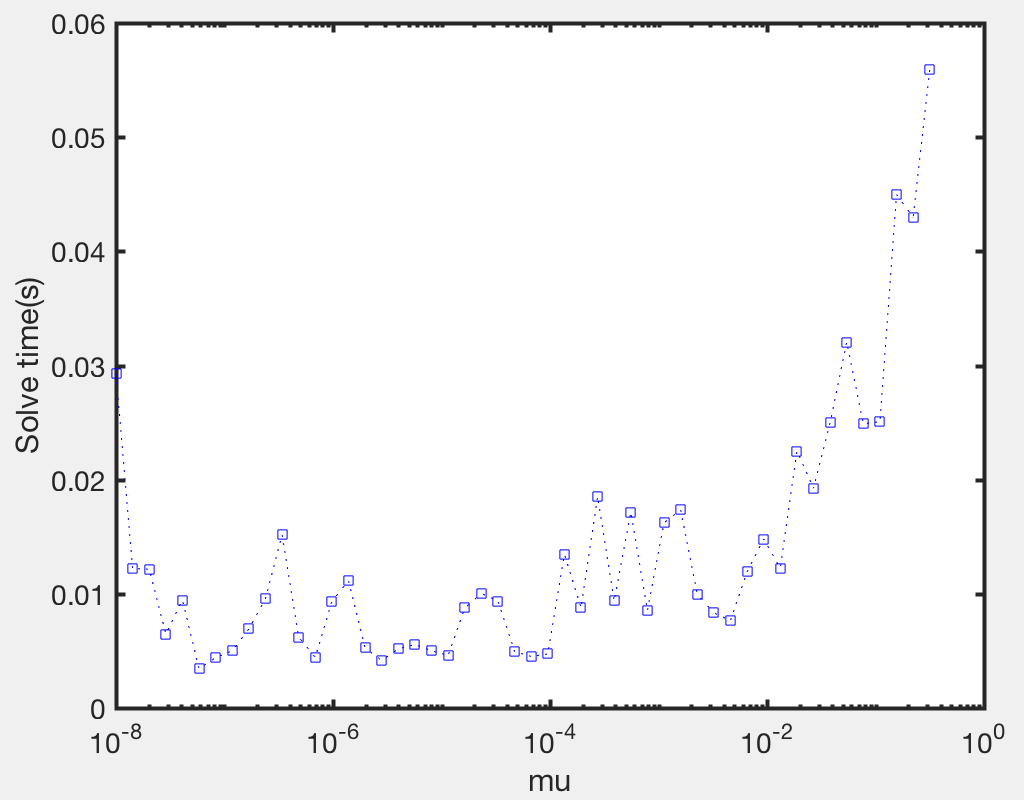
\includegraphics[width=\linewidth]{mu_time}
				\caption{Convergence time with respect to $\mu$}
				\label{n12}
			\end{minipage}
			\begin{minipage}{0.5\linewidth}
				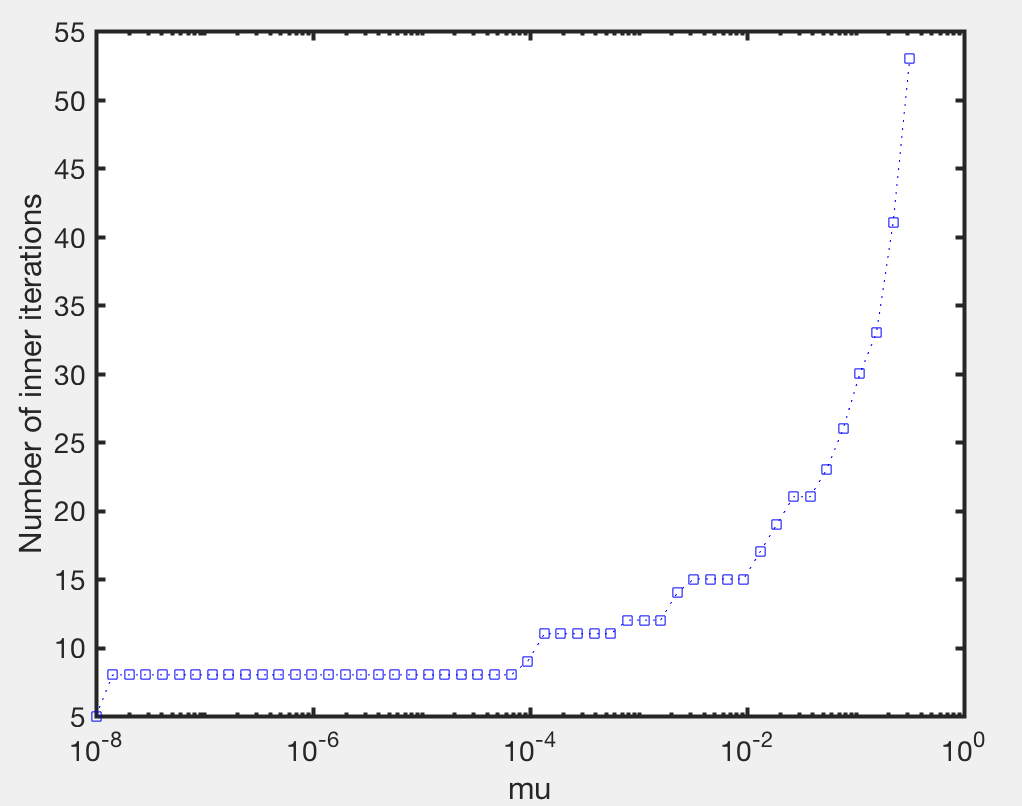
\includegraphics[width=\linewidth]{mu_it}
				\caption{Inner iterations number with respect to $\mu$}	
				\label{n8}			
			\end{minipage}
		\end{figure}
		
		\paragraph{} We note, as discussed hereinbefore, that for smaller values of $\mu$, we reach convergence \textcolor{red}{faster} than for greater (close to $1$) values. However, we can note that for very small values of $\mu$ ($\simeq \eps = 10^{-8}$), convergence is not reached since $\kappa$ is believed to be 0 : after one more outer loop, the algorithm stops (since $\kappa$ remains the same, and so for the  corresponding optimization problem). Hence, the first value of the different plots have to be treated with caution, since they do not correspond to fully solved optimization problems. 
		
				\begin{figure}[h!]
			\begin{minipage}{0.5\linewidth}
				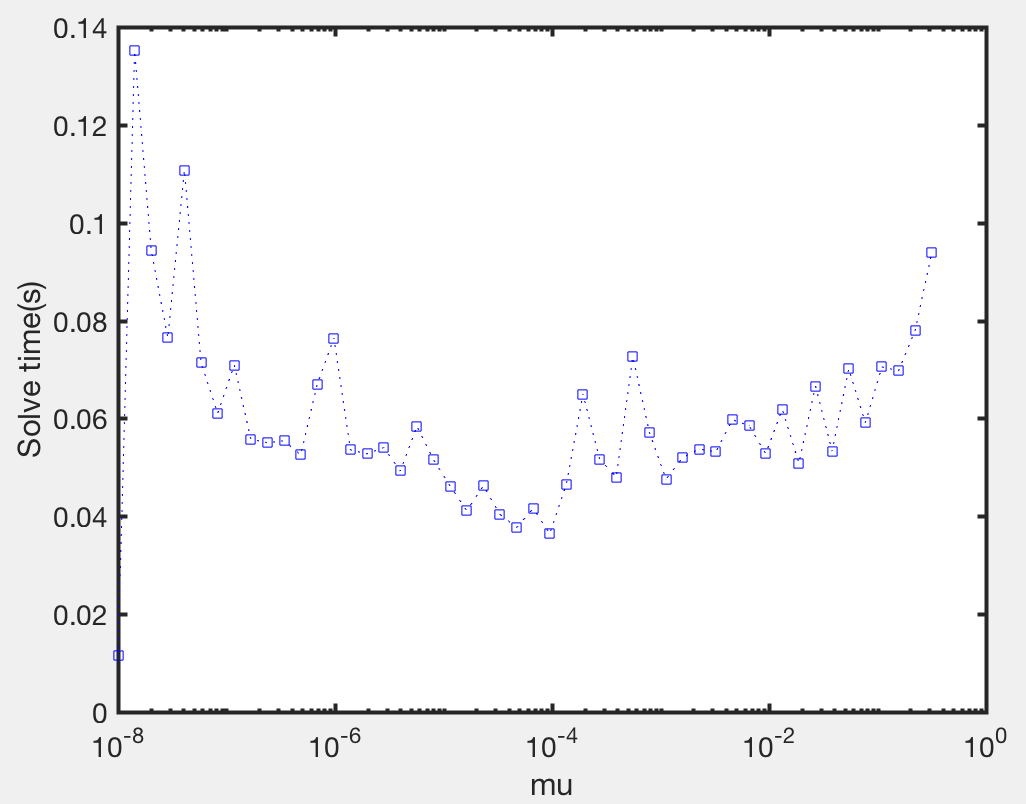
\includegraphics[width=\linewidth]{mu_time_50}
				\caption{Convergence time with respect to $\mu$, $d=50$}
				\label{mu_time_50}
			\end{minipage}
			\begin{minipage}{0.5\linewidth}
				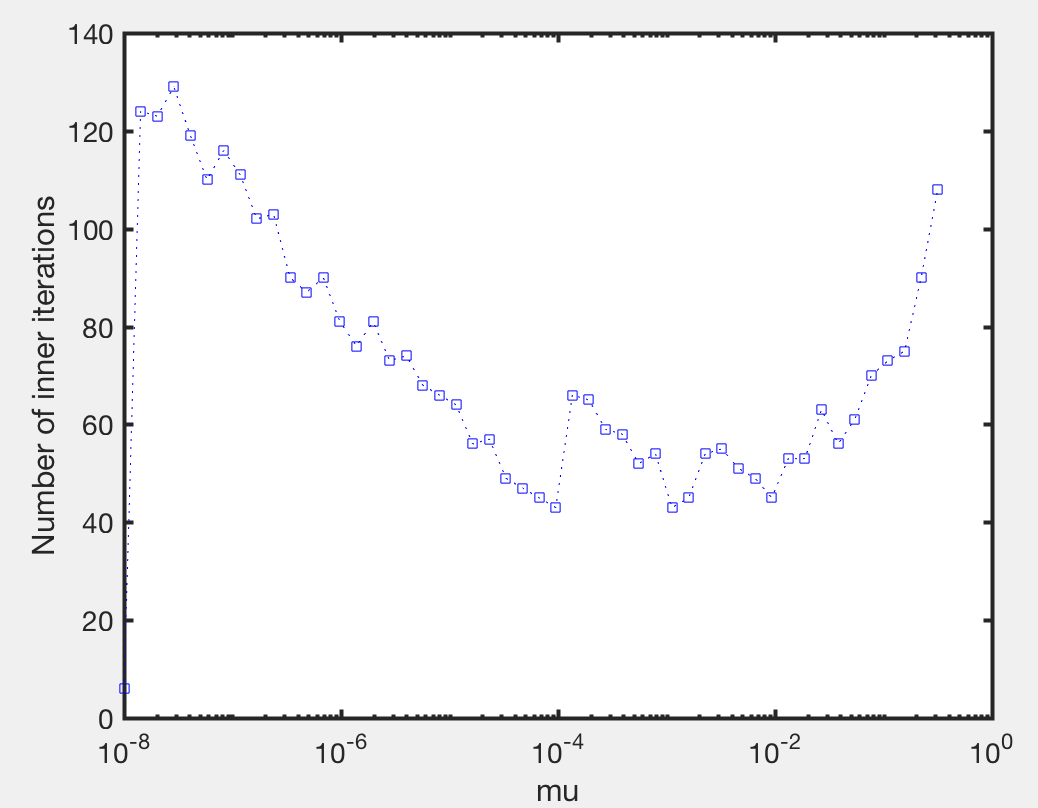
\includegraphics[width=\linewidth]{mu_it_50}
				\caption{Inner iterations number with respect to $\mu$, $d=50$}	
				\label{mu_it_50}			
			\end{minipage}
		\end{figure}
		
		\paragraph{} We can repeat that experiment for a state space of dimension 50. We expect the computation time to be bigger (due to the resolution of a 50*50 system, instead of a 2*2). As shown if figure (\ref{mu_time_50}), the computation time is indeed higher. If one can naively expect a solving time ratio of $\frac{50^3}{2^3}$ (naive cost of inverting the Hessian), this does not show that expressively here since this operation is not the longest one performed by Matlab (Matlab solves the system using precompiled code, while its interpreter still has to iterate through our loop). We also expect the number of iterations needed for solving the problem to be larger since there are more independent directions to explore, which is confirmed by figure (\ref{mu_it_50}). 
		

	}


\end{document}